% This is samplepaper.tex, a sample chapter demonstrating the
% LLNCS macro package for Springer Computer Science proceedings;
% Version 2.20 of 2017/10/04
%
\documentclass[runningheads]{llncs}
%
\usepackage{times}
\usepackage{soul}
\usepackage{url}
\usepackage[hidelinks]{hyperref}
\usepackage[utf8]{inputenc}
\usepackage[small]{caption}
\usepackage{graphicx}
\usepackage{amsmath}
\usepackage{booktabs}
\usepackage{bbm}
\urlstyle{same}
% Used for displaying a sample figure. If possible, figure files should
% be included in EPS format.
%
% If you use the hyperref package, please uncomment the following line
% to display URLs in blue roman font according to Springer's eBook style:
% \renewcommand\UrlFont{\color{blue}\rmfamily}

\begin{document}
%
\title{INForex: Interactive News Digest for Forex Investors}
%
%\titlerunning{Abbreviated paper title}
% If the paper title is too long for the running head, you can set
% an abbreviated paper title here
%
\author{Chih-Hen Lee\inst{1}\and
Yi-Shyuan Chiang\inst{2} \and
Chuan-Ju Wang\inst{3}}
%
\authorrunning{Lee et al.}
% First names are abbreviated in the running head.
% If there are more than two authors, 'et al.' is used.
%
\institute{Research Center for Information Technology Innovation, \\Academia Sinica, Taipei, Taiwan\\
\email{\{\inst{1}ch.lee, \inst{3}cjwang\}@citi.sinica.edu.tw} \\
\email{\inst{2}yschiang@gapp.nthu.edu.tw}
\\}
%
\maketitle              % typeset the header of the contribution
%
\vspace{-0.6cm}
\begin{abstract}
As foreign exchange (Forex) markets reflect real-world events, locally or globally, financial news is often leveraged to predict Forex trends. 
In this demonstration, we propose INForex, an interactive web-based system that displays a Forex plot alongside related financial news. To our best knowledge, this is the first system to successfully align the presentation of two types of time-series data---Forex data and textual news data---in a unified and time-aware manner and as well as the first Forex-related online system leveraging deep learning techniques. 
The system can be of great help in revealing valuable insights and relations between the two types of data and is thus valuable for decision making not only for professional financial analysts or traders but also for common investors.
The system is available online at~\url{http://chlee.pythonanywhere.com/forex/}, and the introduction video is at~\url{https://youtu.be/ZhFqQamTFY0}.

\keywords{FOREX  \and Attention Mechanism \and Web System.}
\end{abstract}
%
%
%
\vspace{-0.8cm}
\section{Introduction}
\vspace{-0.3cm}
Forex markets are influenced by numerous factors, including gross domestic product (GDP), interest rates, and politics.
In order to consider as many factors as possible to gain a more comprehensive view for Forex investment, most investors stay informed by relying on news.

Considering the critical role of news for Forex investment, in this demonstration, we propose INForex, an interactive web-based system that displays a Forex plot alongside related financial news. With the proposed system we seek to align the timing of Forex and news data to highlight the connection between these two types of time-series data. In INForex the release time of news stories is displayed as vertical lines on the Forex plot to emphasize the order of breaking news and exchange rates. Also, when users hover on a vertical line, the background color of the corresponding news will change. 

Moreover, we propose using two event detection methods based on the standard deviation (SD) and directional change (DC)~\cite{7850020} of the Forex data to locate specific periods during which the prices or trends in Forex markets change dramatically.
Via this design, we assist users to make trading strategies by putting the focus on changes of trend or periods of large price volatility.
In addition, with the great advancement in natural language processing (NLP) and deep learning (DL) in recent years, in the proposed system, we utilize attention mechanisms~\cite{attention} to further exploit the semantics in financial news.
Specifically, by leveraging the financial news as training corpus and the aforementioned DC events as labels, our proposed system train an attention-based classification model that can be used to highlight worth-noting news and the potential keywords to users.
Last but not least, INForex also comes with a keyword filtering function that allows users to filter news with self-defined keywords, where they can focus on searching related news of their interests.

To our best knowledge, this is the first system that effectively visualizes these two types of time-series data---Forex data and textual news data---in a unified and time-aware manner and as well as the first Forex system leveraging deep learning techniques. 
The proposed INForex can be of great help in revealing valuable insight and relations between the two types of data and is thus valuable for decision-making not only for professional financial analysts or traders but also for common investors.

\vspace{-0.5cm}
\section{System Description}\label{sec:system}
\vspace{-0.9cm}
\begin{figure}
  \centering
  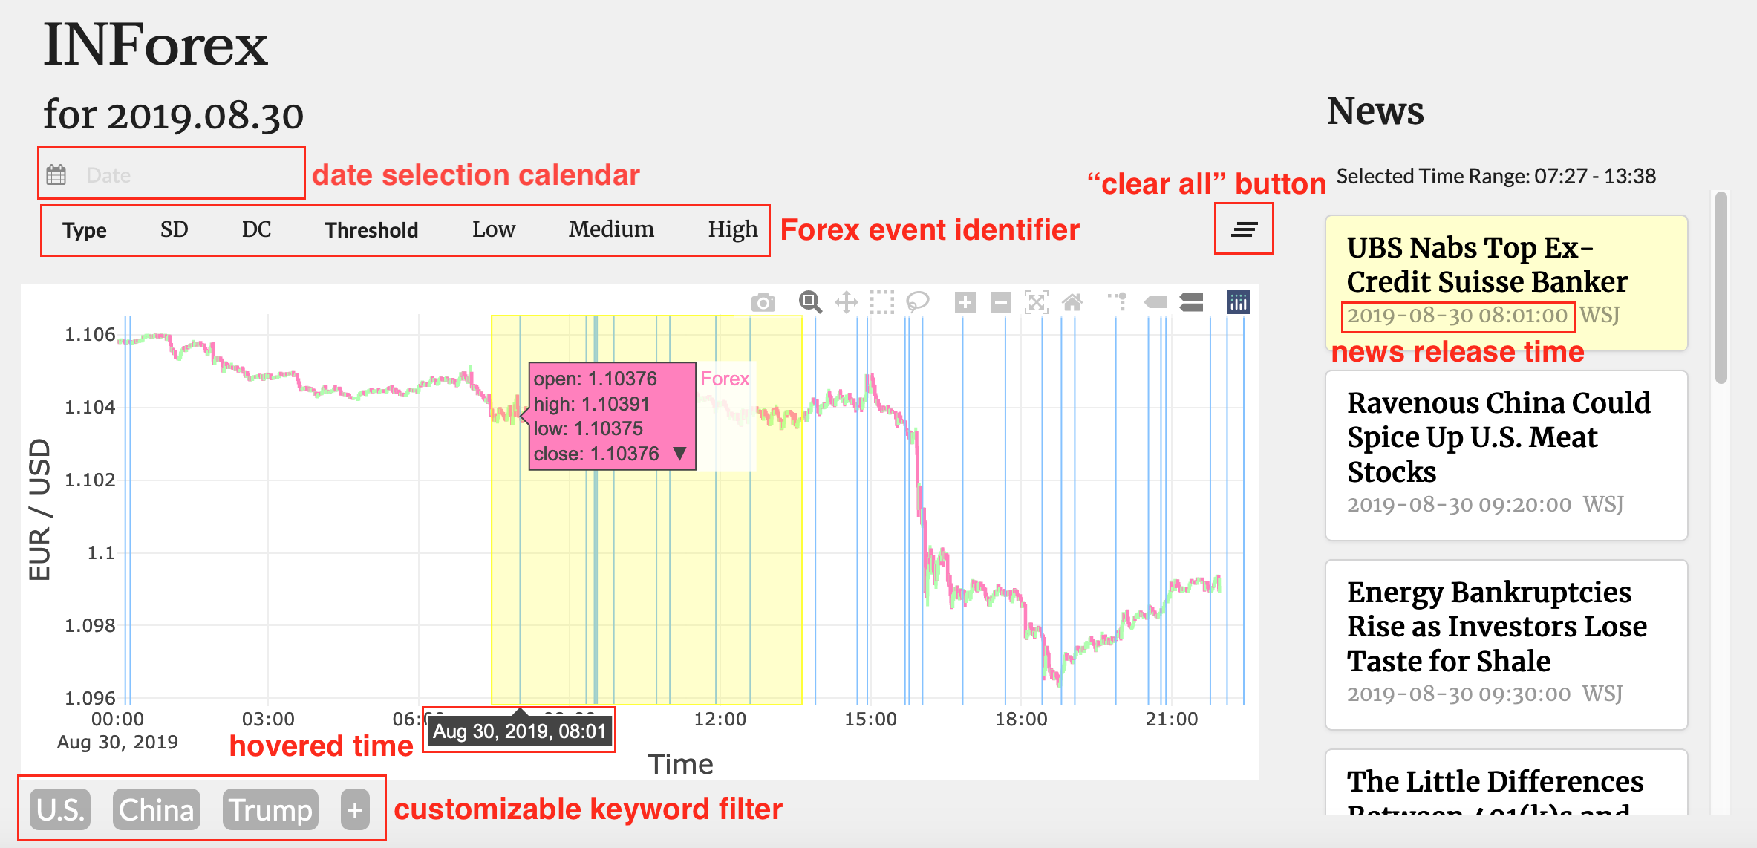
\includegraphics[width=0.7\textwidth]{hover.pdf}
  \caption{The interfaces of INForex. Note that news is highlighted when the cursor hovers over the
  corresponding timeline on the chart.}
  \label{fig:hover}
\end{figure}\
\vspace{-1.7cm}

\subsection{Data Collection}
\vspace{-0.3cm}
The Forex data was collected from
philipperemy/FX-1-Minute-Data.\footnote{\url{https://github.com/philipperemy/FX-1-Minute-Data}}
The training period is from January 1, 2010 to December 31, 2018, and the testing period is from August 4, 2019 to September 13, 2019 (which is the time span shown in the system). 

As for news, we crawled articles from The Wall Street
Journal,\footnote{\url{https://www.wsj.com}}. Following the above setting, we separate these news into training, validation, and testing sets, the number of news corresponds to which are 80,000, 2,766, and 1,021, respectively
Note that the validation set is the last 2,766 news in the training period, and only the testing batch of news is displayed on our system.
\vspace{-0.5cm}
\subsection{Event Detection Algorithms}\label{sec:algo}
\vspace{-0.2cm}
The proposed system comes with two event detection algorithms: one based on
the standard deviation of Forex price differences (referred as SD events hereafter) and one based on the directional change of Forex prices (referred
as DC events hereafter)~\cite{7850020}. 
Specifically, SD events indicate time points during which the Forex prices
dramatically change, whereas DC events show time points where the trends of
Forex prices change.

We here briefly describe the two algorithms.
Let $P= [p_1, p_2, ..., p_n]$ denote a series of Forex prices, where $p_t$
stands for the CLOSE Bid Quote at minute~$t$ and $n$ equals the total
numbers of daily Forex data; also, the series of difference rates between two
Forex prices is defined as $\mathcal{D}= [d_1, d_2, ..., d_m]$, where $d_t =
{(p_{t+w}-p_t)}/{p_t}$ and $w\in\mathbbm{Z}^+$ denotes the range in minutes.
Note that we set $w=20$ in our prototype system.
We first calculate the standard deviation of differences in list~$\mathcal{D}$
and denote this as $\sigma_\mathcal{D}$; we then use the $z$-score of each
difference to determine the events (i.e.,
$z_{d_i}=(|d_i-m_{\mathcal{D}}|)/\sigma_{\mathcal{D}}>\tau$), where
$m_{\mathcal{D}}$ denotes the mean of the list~$\mathcal{D}$.)
In this demonstration, we consider $\tau=1,2,3$ as our thresholds 
corresponding to labels \emph{Low}, \emph{Medium}, and \emph{High} in the
system. 
Note that a higher threshold locates fewer events.

As for the DC events, the market is summarized into a set of uptrend and
downtrend events~\cite{7850020}.
A DC event, which includes a start point and an end point, can be seen as a period
during which the trend starts to change.
Initially, we use the first element in the price list~$p_1$ as the starting point; then, the algorithm starts looking through the price list~$P$
in a sequential manner until it locates a price~$p_c$ for which
$|{(p_c-p_1)}/{p_1}|>\theta$.
In this demo, we consider
$\theta=\sigma_{\mathcal{D}},2\sigma_{\mathcal{D}},3\sigma_{\mathcal{D}}$ as
our thresholds, corresponding to labels \emph{Low},
\emph{Medium}, and \emph{High} in the system.
If $p_c > p_1$, the span from $p_1$ to $p_c$ denotes an upward DC event;
otherwise, it is a downward DC event.
After finding the first DC event, we look for other DC events in the
rest of the price sequence.
\vspace{-0.5cm}
\subsection{Attention Model}
\vspace{-0.3cm}
In this subsection, we introduce the pipeline of our model in detail. First, we represent each word in news titles and content with the pre-trained embedding from GloVe.\footnote{\url{https://nlp.stanford.edu/projects/glove/}}
We later construct an attention layer~\cite{attention}
to aggregate the words embeddings in each news into one document embedding for each news.
According to~\cite{attention}, the attention mechanism is formulated as ${\rm Attention}(Q, K, V) = {\rm softmax}(QK\textsuperscript{T}/\sqrt{d_k})V$, where $d_k$ is the dimension of keys and queries. In our settings, the queries($Q$) are initially randomized, while the keys($K$) and values($V$) are the GloVe embeddings for words. Here, the main concept is that every word contributes to the document embeddings by different levels; therefore, if a word accounts for a much greater weight than other words in the document do, it might be a potential keyword. After getting the document embeddings, we first apply a ReLU activation function, and then pass the embeddings to a linear classification layer to predict the final label. In terms of labeling training data, a piece of news is labeled as positive when there is a start of any high-threshold DC event in the interval ${(t, t+30)}$, where $t$ is the news release time in minutes. Otherwise, it will be labeled as negative.

Other experimental details are listed as follows.
We implement the model under the PyTorch\footnote{\url{https://pytorch.org/}} framework. To reduce the training time, we only use the first 200 words in the concatenated news title and content as the textual input. For the training process, we select Adam~\cite{Adam} as the optimizer with learning rate 0.0001, and train data with 120 epochs and batch size 20.
\vspace{-0.5cm}
\subsection{Interfaces and features}
\vspace{-0.3cm}
The INForex interface can be divided into two main parts: 1) the Forex chart
(in the left panel of the system) and 2) the news section (the right panel).

\vspace{-0.2cm}
\subsubsection{Interactive Forex Chart}
\vspace{-0.2cm}
Forex prices are displayed by a standard candlestick chart, powered by
Plotly graphing
libraries.\footnote{\url{https://https://plotly.com/graphing-libraries/}}
Users can specify the date they are interested in with the calendar icon above
the chart and then explore the chart freely by zooming in or dragging out the
time frame of interest.
Except for the Forex chart, the blue vertical lines correspond to the news story
release time points. 
As shown in Figure~\ref{fig:hover}, the corresponding news in the right panel
is highlighted if users hover over the corresponding blue line on the chart.
Moreover, users can easily spot specific time ranges of interest
by single-clicking the start and end points of a period on the Forex chart
(resulting in the yellow span in the figure); the news section in the right
panel changes correspondingly according to the selected time span.

\vspace{-0.4cm}
\subsubsection{Forex Event Identifier}
\vspace{-0.2cm}
Users specify event types (i.e., SD or DC)  and the corresponding thresholds (i.e., Low, Medium, or High) with the Forex event identifier (see the buttoms below the date selection calendar in Figure~\ref{fig:hover}), after which the algorithm output is shown on the Forex chart as
gray dots for the SD events and span lines for the DC events.
Note that once done with a specific setting, users clear the setting with
the ``clear all'' button on the top-right of the left panel;
a higher threshold locates fewer events.

\subsubsection{Attention Weight Visualization}
\vspace{-1.3cm}
\begin{figure*}
  \centering
  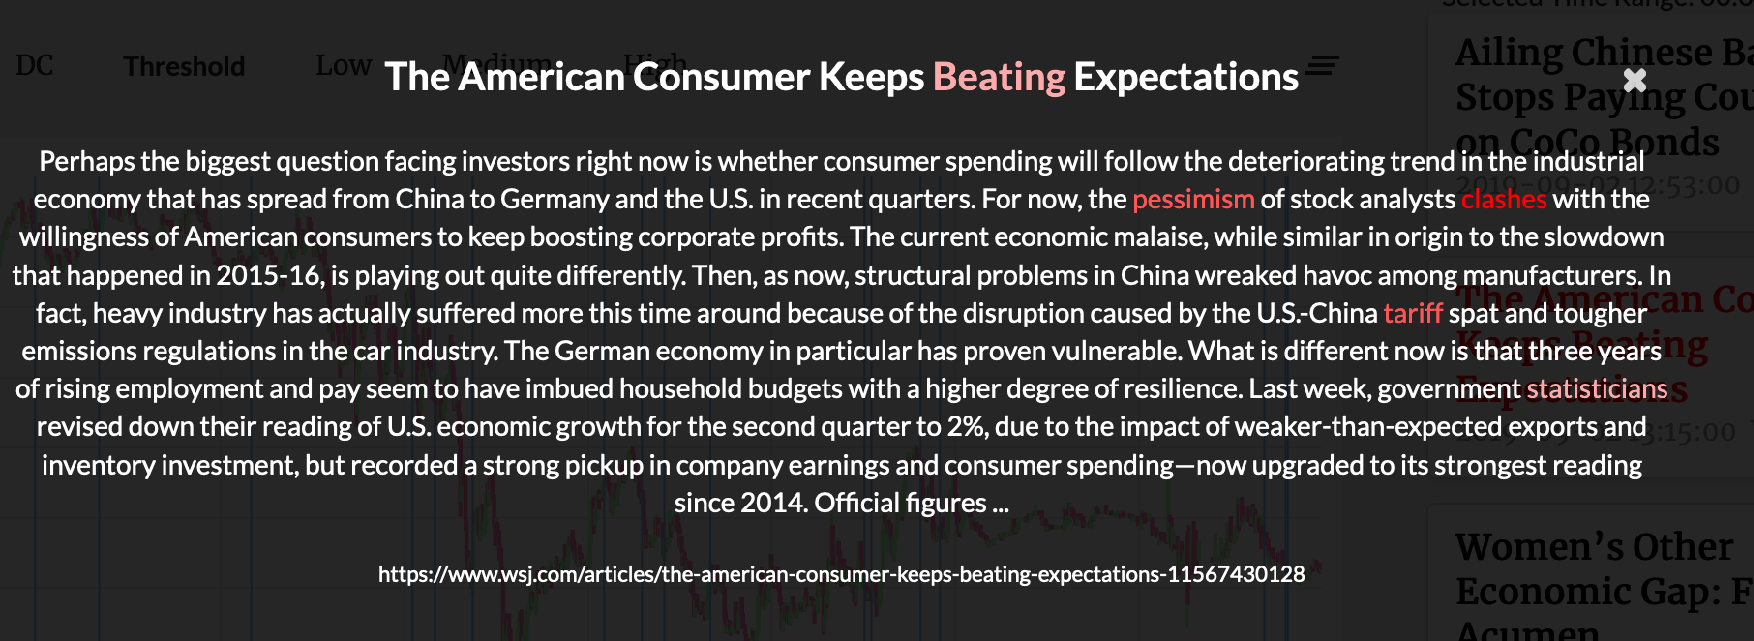
\includegraphics[width=0.7\linewidth]{weights.pdf}
  \caption{Attention weights. The word ``clashes'' is a dark red word, ``pessimism'' and ``tariff'' are red words, and ``Beating'' and ``statisticians'' are pink words.}
  
  \label{fig:weights}
\end{figure*}
\vspace{-0.7cm}
If a news is predicted as positive (i.e., potentially highly correlated with the DC events), the news title is highlighted in red.
After clicking the positive news title, a window showcasing the news title and content with highlighted keywords will pop up.
Here, three classes of keywords are defined. Let $\ell$ be the word count of a concatenated news title and content, and the maximum of $\ell$ is set to 200 as mentioned above. The dark red words are the most worth-noting words whose attention weights are greater than ${40}/{\ell}$, while the attention weights of red words and pink words are greater than ${20}/{\ell}$ and ${10}/{\ell}$, respectively.
As shown in Figure~\ref{fig:weights}, our model is able to capture keywords related to the Forex market in this case.
\vspace{-0.5cm}
\section{Conclusion and Future Work}\label{sec:conclude}
\vspace{-0.3cm}
In this paper, we propose INForex, an interactive system that aligns the Forex data and textual news data in a unified and
time-aware manner.
By placing the chart and related news side by side and displaying the potential keywords, users, financial
professionals, and amateur investors can all understand Forex trends
quicker and easier.

With limited financial resources, we can only propose a static prototype system with data made available online. However, since the real-time feature is crucial for investors, we will thrive to make INForex become a real-time system in the future, either with real-time industrial APIs.
We hope that this demonstration can facilitate more research on predicting Forex markets through deep learning models in the future.

%
% ---- Bibliography ----
%
% BibTeX users should specify bibliography style 'splncs04'.
% References will then be sorted and formatted in the correct style.
%
% \bibliographystyle{splncs04}
% \bibliography{mybibliography}
%
\begin{thebibliography}{8}

\bibitem{7850020}
Amer Bakhach and Edward P. K. Tsang and Hamid Jalalian: Forecasting directional changes in the FX markets. In: Proceedings of the 2016 IEEE Symposium Series on Computational Intelligence (SSCI), pp. 1--8. (2010)

\bibitem{attention}
Vaswani, Ashish and Shazeer, Noam and Parmar, Niki and Uszkoreit, Jakob and Jones, Llion and Gomez, Aidan N and Kaiser, \L ukasz and Polosukhin, Illia: Attention is All you Need. In: Proceedings of the 31st International Conference on Neural Information Processing Systems (NeurIPS), pp. 6000--6010. (2017)

\bibitem{Adam}
Diederik P. Kingma and Jimmy Ba: Adam: A Method for Stochastic Optimization. In: Proceedings of the 3rd International Conference on Learning Representations (ICLR) (2015)


\end{thebibliography}
\end{document}
